%%% Folie
\begin{frame}{Lernziele}
    \begin{itemize}
       \item Interrupts als alternative Methode nutzen können, um Sensorwerte auszulesen
       \item  Bedeutung von Zeitstempeln
        \item Möglichkeiten zum Abspeichern von Sensorwerten kennenlernen
    \end{itemize}
\end{frame}


 %-------------------------------------------------------------------------------
\section{Interruptbasierte Programmierung}
%-------------------------------------------------------------------------------

%%% Folie
\begin{frame}{Was ist ein Interrupt?}
    \begin{itemize}
        \setlength{\itemindent}{1.2in}
        \item [\textbf{Definition Interrupt}]
    \end{itemize}

    \begin{itemize}
        \item Allgemein: Signal zur CPU, das den aktuellen Prozess unterbricht mittels eines  \textcolor{blue}{\textbf{Interrupt Requests}}
        \item Signal kann durch Software generiert werden oder hardwareseitig via I/O Device
        \item Zur Behandlung wird eine sogenannte \textcolor{blue}{\textbf{Interrupt Service Routine (ISR)}} aufgerufen, ähnlich wie eine Callback Funktion
     \end{itemize}
\end{frame}

\begin{frame}{Signalzustände 1}
    \begin{itemize}
        \setlength{\itemindent}{2.5in}
        \item [\textbf{Signalzustände als Auslöser}]
    \end{itemize}
    \begin{figure}[!htb]
        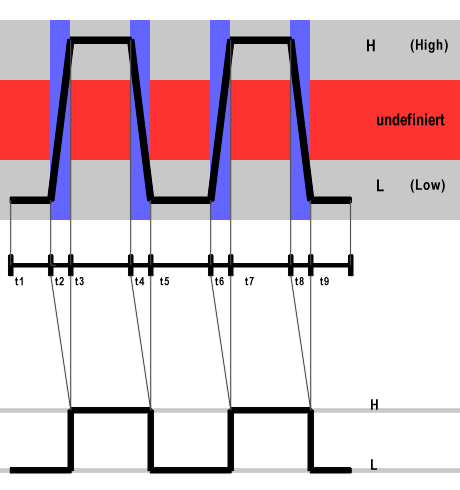
\includegraphics[scale=0.5]{4-python2/img/DigSig2}
    \end{figure}
\end{frame}



\begin{frame}{Signalzustände 2}
    \begin{itemize}
        \setlength{\itemindent}{1.6in}
        \item [\textbf{Signalzustände und GPIO}]
    \end{itemize}
   \begin{itemize}
        \item GPIO Pins dienen als Auslöser (Interrupt Sources)
        \item Im Rahmen einer simplen Synchronisation basiert das Sampling standardmäßig auf einem 3er-Zyklus (z.B. 1 $\rightarrow$ 0 $\rightarrow$ 0 oder 0 $\rightarrow$ 1 $\rightarrow$ 1)
        \item Jeder PIN kann konfiguriert werden für: Level-sensitive (High/Low), Steigende/fallende Flanke, Asynchron  (steigende/fallende Flanke)
     \end{itemize}

\end{frame}




 %-------------------------------------------------------------------------------
\section{Zeitstempel}
%-------------------------------------------------------------------------------

%%% Folie
\begin{frame}{Wozu werden Zeitstempel benötigt?}
    \begin{itemize}
        \setlength{\itemindent}{1.9in}
        \item [\textbf{Wesentliche Funktionen im IoT}]
    \end{itemize}

    \begin{itemize}
        \item Protokollierung von Ereignissen
        \item Tracing von Nachrichten
        \item Speichern von Sensorwerten als Historie
        \item Programmierung von Ablauflogiken
        \item ...
     \end{itemize}
\end{frame}


\begin{frame}[fragile]{Zeitstempel - Logging 1}
    \begin{itemize}
        \setlength{\itemindent}{1.9in}
        \item [\textbf{Protokollierung von Ereignissen}]
    \end{itemize}

    \begin{itemize}
              \item Log Files enthalten Informationen über den zeitlichen Ablauf des Programmes
               \item Fehler können in einen zeitlichen Zusammenhang gebracht werden
     \end{itemize}

    \begin{lstlisting}[language=Python, gobble=8]
        # Logging Konfigurieren mittels JSON Datei
           import os
           import json
           import logging.config
           def setup_logging(default_path='config/logging.json', default_level=logging.INFO, env_key='LOG_CFG'):
              path = default_pat
              dirname = os.path.dirname(__file__)
              filename = os.path.join(dirname, path)
              value = os.getenv(env_key, None)
              if value:
                path = value
              if os.path.exists(filename):
                 with open(filename, 'rt') as f:
                   config = json.load(f)
                   logging.config.dictConfig(config)
              else:
                   logging.basicConfig(level=default_level)
        \end{lstlisting}
\end{frame}

\begin{frame}[fragile]{Zeitstempel - Logging 2}
    \begin{itemize}
        \setlength{\itemindent}{1.4in}
        \item [\textbf{Konfiguration der Logger}]
    \end{itemize}

    \begin{itemize}
         \item Verschiedene Handler für Ausgaben möglich (Files, Console, Monitoring Server im Netz etc.)
         \item Zeitstempel lassen sich über Formatter konfigurieren
     \end{itemize}

    \begin{lstlisting}[language=Java, gobble=8]
         // Logging Konfiguration aus der Datei: config/logging.json
           {   "version": 1,
               "disable_existing_loggers": false,
               "formatters": {
                    "simple": {
                       "format": "%(asctime)s - %(name)s - %(levelname)s - %(message)s"
                    }
                },
               "handlers": {
                    "info_file_handler": {
                        "class": "logging.handlers.RotatingFileHandler",
                        "level": "INFO",
                        "formatter": "simple",
                        "filename": "my_app.log",
                        "maxBytes": 10485760,
                        "backupCount": 5,
                        "encoding": "utf8"
                  }
               "root": {
                    "level": "INFO",
                    "handlers": ["info_file_handler"]
               }
          }
        \end{lstlisting}
\end{frame}


\begin{frame}[fragile]{Zeitstempel - Tracing}
    \begin{itemize}
        \setlength{\itemindent}{1.4in}
        \item [\textbf{Tracing von Nachrichten}]
    \end{itemize}

    \begin{itemize}
              \item Idee: Daten auf einem Gerät A zum Zeitpunkt x erfassen und als Nachricht versenden
               \item Gerät B (z.B. ein weiterer Raspberry Pi oder ein Server) soll die Nachricht erhalten
               \item Zeitstempel wird auf Gerät A an eine zu übertragende Nachricht angehängt
               \item Wenn Gerät B die Nachricht erhält, kann dort ermittelt werden, von wann die Nachricht ist (z.B. im Log von Gerät B nachschauen)
     \end{itemize}

\end{frame}


\begin{frame}[fragile]{Zeitstempel - Format 1}
    \begin{itemize}
        \setlength{\itemindent}{2.4in}
        \item [\textbf{Wie sollten Zeitstempel formatiert sein?}]
    \end{itemize}

    \begin{itemize}
              \item Aktuell 38 verwendete Zeitzonen weltweit (siehe \url{https://www.timeanddate.com/time/current-number-time-zones.html})
               \item ISO 8601 als Standard für Formatierung menschenlesbarer Zeitstempel
               \item Beispiel: 2019-10-31T16:56:34.297+02:00 $\rightarrow$ Uhrzeit inkl. Millisekunden vom 31 Oktober, 2 Stunden "Offset" auf die UTC Weltzeit addiert
               \item Gewöhnlich werden die Daten zu UTC formatiert, also hier 2019-10-31T14:56:34.297+00:00 oder auch Zulu-Zeit: 2019-10-31T14:56:34.297Z
               \item Mit UTC/Zulu kann überall eine lokale Uhrzeit ermittelt werden, wir müssen also für die Deutsche Sommerzeit +2 Stunden auf den UTC Zeitstempel addieren
     \end{itemize}
       \begin{lstlisting}[language=Python, gobble=8]
        # Beispiel: aktuellen Zeitstempel nehmen und ausgeben
           from datetime import datetime,timezone

           current_timestamp = print(datetime.now(timezone.utc).isoformat(timespec='milliseconds')) # aktueller Zeitstempel
           #  Ausgabe bspw: 2019-10-31T10:42:16.634+00:00
        \end{lstlisting}

\end{frame}

\begin{frame}[fragile]{Zeitstempel - Format 2}
    \begin{itemize}
        \setlength{\itemindent}{2.4in}
        \item [\textbf{Aber woher bekommen wir den Offset?}]
    \end{itemize}

    \begin{itemize}
              \item  Den Offset könnte man fest einstellen, wenn man weiß, wo das Gerät voraussichtlich aufgestellt sein wird
               \item Besser: UTC Zeitstempel holen von einem Remote Server
               \item Hier kommt das NTP Protokoll zum Einsatz (siehe \url{https://tools.ietf.org/html/rfc5905})
               \item Der Raspberry kann systemseitig mit NTP synchronisieren
               \item Auch möglich: NTP Client via pip install ntplib
    \end{itemize}
\end{frame}

\begin{frame}[fragile]{Zeitstempel - Format 3}
    \begin{itemize}
        \setlength{\itemindent}{2.4in}
        \item [\textbf{}]
    \end{itemize}

  \begin{lstlisting}[language=Python, gobble=8]
        # Beispiel: Zeitstempel via NTP Client abrufen und formatieren
           import ntplib
           import pytz
           from time import ctime
           from datetime import datetime,timezone

           client = ntplib.NTPClient()
           response = client.request('ptbtime1.ptb.de') # Request an die Physikalisch Technische Bundesanstalt (PTB) in Braunschweig
           response_timestamp = response.tx_time # Zeitstempel unformatiert als float

           timestamp_utc_from_ntp = datetime.fromtimestamp(response_timestamp, timezone.utc).isoformat(timespec='milliseconds') # UTC
           timestamp_zulu = timestamp_utc_from_ntp[:-6] + 'Z' # ZULU
           timestamp_local = datetime.fromtimestamp(response_timestamp, pytz.timezone('Europe/Berlin')).isoformat(timespec='milliseconds') # +2 Stunden Offset

           print('UTC:',timestamp_utc_from_ntp, '\n', 'Zulu:',timestamp_zulu, '\n', 'Local:',timestamp_local)

           """ Ausgabe bspw: UTC: 2019-10-20T18:42:16.634+00:00
                                         Zulu: 2019-10-20T18:42:16.634Z
                                         Local: 2019-10-20T20:42:16.634+02:00
           """
        \end{lstlisting}

\end{frame}


\section{Abspeichern von Sensordaten}

%%% Folie
\begin{frame}{Persistenz für Messwerte 1}
    \begin{itemize}
        \setlength{\itemindent}{1.9in}
        \item [\textbf{Warum Messwerte speichern? }]
    \end{itemize}

    \begin{itemize}
        \item Es gibt viele Szenarios, in denen Messwerte auch (lange) nach der Erfassung nützlich sind
        \item Messwerte als Historie/ Zeitfolge abspeichern, z.B. für Aggregation von Temperaturwerten
        \item Messwerte in die Cloud versenden und dazu Puffern (Ringspeicher, der bei Erreichen seiner Kapazität, z.B. 4 GB, zurückgesetzt wird)
        \item Messwerte mathematisch anpassen, z.B. mittels Machine Learning Modellen
        \item Ereignisse auslösen, wenn eine bestimmte Anzahl Messwerte erreicht wird (z.B. Dauer der Unterbrechung einer IR-Lichtschranke)
     \end{itemize}
\end{frame}


\begin{frame}{Persistenz für Messwerte 2}
    \begin{itemize}
        \setlength{\itemindent}{1.9in}
        \item [\textbf{Welche Möglichkeiten gibt es? }]
    \end{itemize}

    \begin{itemize}
        \item Beliebt und einfach ist das Abspeichern der Messwerte im CSV Format (Comma Separated Values)
        \item Vorteile: Schnell aufgesetzt, Ausgabedatei ist universell verwendbar, z.B. mit Excel
        \item Nachteile: Handling der Relation von Messdaten ist weniger komfortabel, z.B:  Anzahl, Höchstwert, Sortierung
        \item Deswegen bieten sogenannte Embedded Databases eine gute Alternative
        \item Hierzu ist SQLite3 eine häufig verwendete Software (siehe \url{https://www.sqlite.org/about.html}
        \item Vorteile: Daten Handling
        \item Nachteile: Daten nicht ohne Editor einsehbar, Overhead beim Aufsetzen (Tabellen, IO)
     \end{itemize}
\end{frame}

\begin{frame}[fragile]{Persistenz für Messwerte 3}
    \begin{itemize}
        \setlength{\itemindent}{2.4in}
        \item [\textbf{Beispiel zu CSV}]
    \end{itemize}
       \begin{lstlisting}[language=Python, gobble=8]
         # Beispiel zum Schreiben von 3 Messwerten in eine CSV Datei
         from time import sleep
         from datetime import datetime,timezone
         import csv

         def current_timestamp(): # Funktion für den aktuellen Zeitstempel inklusive 1 Sekunde Pause
          sleep(1)
          return datetime.now(timezone.utc).isoformat(timespec='milliseconds')

         # Messung als Tupel aus Zeitstempel und Messwert
         measurements = [(current_timestamp(), 0.65),(current_timestamp(), 0.7),(current_timestamp(), 0.98) ]

         with open('messdaten.csv', 'a', newline='') as f:  # Öffne die messdaten.csv Datei und schreibe ans Ende
           writer = csv.writer(f)
           writer.writerows(measurements)
        \end{lstlisting}

\end{frame}




\begin{frame}[fragile]{Persistenz für Messwerte 4}
    \begin{itemize}
        \setlength{\itemindent}{2.4in}
        \item [\textbf{Beispiel zu SQLite DB}]
    \end{itemize}
       \begin{lstlisting}[language=Python, gobble=8]
              # Basierend auf  https://pynative.com/python-sqlite
              # Beispiel zum Schreiben von 3 Messwerten in eine SQLite DB Datei, Modul db.db_helper.py
              import sqlite3
              from sqlite3 import Error

              database = r"sensors.db"

	            def create_connection(db_file): # Verbindung herstellen
                connection = None
                try:
                   connection = sqlite3.connect(db_file)
                   return connection
                except Error as error:
                   print(error)
                return connection

              def create_table(connection, create_table_sql): # Tabelle erstellen
               try:
                  cursor = connection.cursor()
                  cursor.execute(create_table_sql)
               except Error as error:
                  print(error)


        \end{lstlisting}

\end{frame}


\begin{frame}[fragile]{Persistenz für Messwerte 5}
       \begin{lstlisting}[language=Python, gobble=8]
              # Basierend auf  https://pynative.com/python-sqlite
              # Fortsetzung: Modul db.db_helper.py - DB erstellen
                 def create_db():
                    sql_create_measurements_table = """ CREATE TABLE IF NOT EXISTS measurements (
                                        id integer PRIMARY KEY,
                                        timestamp DATETIME,
                                        sensor_value INTEGER); """

                    connection = create_connection(database)

                    if connection is not None:
                       create_table(connection, sql_create_measurements_table)
                    else:
                       print("Fehler! Verbindungsaufbau gescheitert.")

        \end{lstlisting}

\end{frame}


\begin{frame}[fragile]{Persistenz für Messwerte 6}
       \begin{lstlisting}[language=Python, gobble=8]
              # Basierend auf  https://pynative.com/python-sqlite
              # Fortsetzung: Modul db.db_helper.py - Messwerte speichern
                 def save_measurement(measurement): # measurement ist Tupel (Zeitstempel, Messwert)
                    try:
                       connection = create_connection(database)
                       cursor = connection.cursor()
                       print("Verbindung offen.")

                       sqlite_insert_query = """INSERT INTO `measurements`
                            ('id', 'timestamp', 'sensor_value')
                            VALUES (NULL, ?, ?);""" # Null für Autoincrement

                       cursor.execute(sqlite_insert_query, measurement)
                       connection.commit()
                       print("Einfügen erfolgreich für %s Datensätze: ", cursor.rowcount)
                       cursor.close()
                    except sqlite3.Error as error:
                       print("Fehler beim Einfügen", error)
                    finally:
                       if (connection):
                          connection.close()
                          print("Verbindung geschlossen")
       \end{lstlisting}

\end{frame}

\begin{frame}[fragile]{Persistenz für Messwerte 6}
       \begin{lstlisting}[language=Python, gobble=8]
              # Basierend auf  https://pynative.com/python-sqlite
              # Fortsetzung: Modul db.db_helper.py - Messwerte lesen
                 def read_measurements():
                    results = []
                    try:
                       connection = create_connection(database)
                       cursor = connection.cursor()
                       sqlite_select_query = """SELECT * from measurements"""
                       cursor.execute(sqlite_select_query)
                       records = cursor.fetchall()
                       print("%s Messwerte gefunden", len(records))
                       for row in records:
                          results.append((row[1], row[2]))# row ist 3-Tupel (ID, Zeitstempel, Messwert)
                       cursor.close()
                       return results
                    except sqlite3.Error as error:
                       print("Fehler beim Lesen aus Tabelle", error)
                    finally:
                       if (connection):
                          connection.close()
       \end{lstlisting}

\end{frame}

\begin{frame}[fragile]{Persistenz für Messwerte 7}
       \begin{lstlisting}[language=Python, gobble=8]
              # Fortsetzung: Verwenden des Moduls db.db_helper.py
                 from time import sleep
                 from datetime import datetime,timezone
                 from db import db_helper

                 def current_timestamp(): # Funktion für Zeitstempel aus CSV Beispiel
                    sleep(1)
                    return datetime.now(timezone.utc).isoformat(timespec='milliseconds')

                 measurements = [(current_timestamp(), 0.65),(current_timestamp(), 0.7),(current_timestamp(), 0.98) ] # Messungen als Tupel

                 db.create_db() # DB anlegen

                 for  measurement in measurements:
                    db.save_measurement((m)). # Alle Messwerte abspeichern

                 measurement_list = db_helper.read_measurements() # Alle Messwerte laden

                 for measurement in measurement_list:  # Alle Messwerte ausgeben
                    print(measurement)
       \end{lstlisting}

\end{frame}
